\documentclass[12pt,letterpaper]{article}
\usepackage[letterpaper,left=0.7in,right=0.7in,top=0.85in,bottom=0.85in,headheight=18pt,headsep=14pt,footskip=0.45in]{geometry}
\usepackage[T1]{fontenc}
\usepackage{newcent}
\usepackage{tikz}
\usepackage{array}
\usepackage{fancyhdr}
\pagestyle{fancy}
\fancyhf{}
\fancyhead[L]{Week 7 / Take-away games / Grades 4--5}
\fancyfoot[L]{Bellingham Math Circle / Week 7}
\fancyfoot[R]{\thepage}
\renewcommand{\headrulewidth}{0.4pt}
\renewcommand{\footrulewidth}{0pt}
\setlength{\parindent}{0pt}
\setlength{\parskip}{0pt}
\newcommand{\prob}[1]{\textbf{Problem #1:}}
\newcommand{\game}[1]{\mbox{\{#1\}}}
\newenvironment{problem}{\par\noindent\begin{minipage}{\linewidth}}{\end{minipage}\par\vspace{0.9cm}}
\begin{document}
In every game in this packet, two players take turns taking counters from a pile. Each problem says how many counters a player may take on a turn. Unless a problem says otherwise, whoever takes the last counter wins.

\vspace{0.7cm}
\begin{problem}
\prob{1} On each turn, a player takes 1, 3, or 4 counters. For each starting pile from 1 to 24, decide whether you would rather go first or second. Shade the box of every pile where you would rather go second. In every other box, write how many counters you could take on your first turn to be sure to win.
\vspace{0.2cm}
\begin{center}
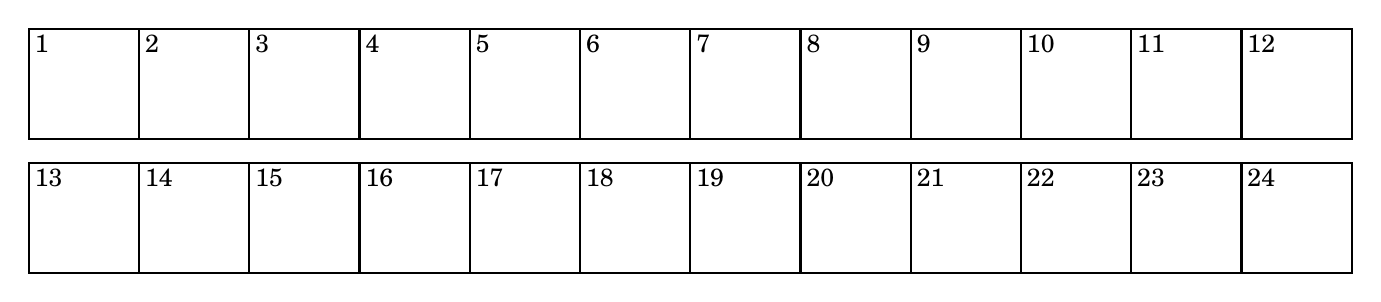
\begin{tikzpicture}
\draw[line width=0.8pt] (0.000,0.000) rectangle (1.400,-1.400);
\node[font=\small,anchor=north west,inner sep=2pt] at (0.000,0.000) {1};
\draw[line width=0.8pt] (1.400,0.000) rectangle (2.800,-1.400);
\node[font=\small,anchor=north west,inner sep=2pt] at (1.400,0.000) {2};
\draw[line width=0.8pt] (2.800,0.000) rectangle (4.200,-1.400);
\node[font=\small,anchor=north west,inner sep=2pt] at (2.800,0.000) {3};
\draw[line width=0.8pt] (4.200,0.000) rectangle (5.600,-1.400);
\node[font=\small,anchor=north west,inner sep=2pt] at (4.200,0.000) {4};
\draw[line width=0.8pt] (5.600,0.000) rectangle (7.000,-1.400);
\node[font=\small,anchor=north west,inner sep=2pt] at (5.600,0.000) {5};
\draw[line width=0.8pt] (7.000,0.000) rectangle (8.400,-1.400);
\node[font=\small,anchor=north west,inner sep=2pt] at (7.000,0.000) {6};
\draw[line width=0.8pt] (8.400,0.000) rectangle (9.800,-1.400);
\node[font=\small,anchor=north west,inner sep=2pt] at (8.400,0.000) {7};
\draw[line width=0.8pt] (9.800,0.000) rectangle (11.200,-1.400);
\node[font=\small,anchor=north west,inner sep=2pt] at (9.800,0.000) {8};
\draw[line width=0.8pt] (11.200,0.000) rectangle (12.600,-1.400);
\node[font=\small,anchor=north west,inner sep=2pt] at (11.200,0.000) {9};
\draw[line width=0.8pt] (12.600,0.000) rectangle (14.000,-1.400);
\node[font=\small,anchor=north west,inner sep=2pt] at (12.600,0.000) {10};
\draw[line width=0.8pt] (14.000,0.000) rectangle (15.400,-1.400);
\node[font=\small,anchor=north west,inner sep=2pt] at (14.000,0.000) {11};
\draw[line width=0.8pt] (15.400,0.000) rectangle (16.800,-1.400);
\node[font=\small,anchor=north west,inner sep=2pt] at (15.400,0.000) {12};
\draw[line width=0.8pt] (0.000,-1.700) rectangle (1.400,-3.100);
\node[font=\small,anchor=north west,inner sep=2pt] at (0.000,-1.700) {13};
\draw[line width=0.8pt] (1.400,-1.700) rectangle (2.800,-3.100);
\node[font=\small,anchor=north west,inner sep=2pt] at (1.400,-1.700) {14};
\draw[line width=0.8pt] (2.800,-1.700) rectangle (4.200,-3.100);
\node[font=\small,anchor=north west,inner sep=2pt] at (2.800,-1.700) {15};
\draw[line width=0.8pt] (4.200,-1.700) rectangle (5.600,-3.100);
\node[font=\small,anchor=north west,inner sep=2pt] at (4.200,-1.700) {16};
\draw[line width=0.8pt] (5.600,-1.700) rectangle (7.000,-3.100);
\node[font=\small,anchor=north west,inner sep=2pt] at (5.600,-1.700) {17};
\draw[line width=0.8pt] (7.000,-1.700) rectangle (8.400,-3.100);
\node[font=\small,anchor=north west,inner sep=2pt] at (7.000,-1.700) {18};
\draw[line width=0.8pt] (8.400,-1.700) rectangle (9.800,-3.100);
\node[font=\small,anchor=north west,inner sep=2pt] at (8.400,-1.700) {19};
\draw[line width=0.8pt] (9.800,-1.700) rectangle (11.200,-3.100);
\node[font=\small,anchor=north west,inner sep=2pt] at (9.800,-1.700) {20};
\draw[line width=0.8pt] (11.200,-1.700) rectangle (12.600,-3.100);
\node[font=\small,anchor=north west,inner sep=2pt] at (11.200,-1.700) {21};
\draw[line width=0.8pt] (12.600,-1.700) rectangle (14.000,-3.100);
\node[font=\small,anchor=north west,inner sep=2pt] at (12.600,-1.700) {22};
\draw[line width=0.8pt] (14.000,-1.700) rectangle (15.400,-3.100);
\node[font=\small,anchor=north west,inner sep=2pt] at (14.000,-1.700) {23};
\draw[line width=0.8pt] (15.400,-1.700) rectangle (16.800,-3.100);
\node[font=\small,anchor=north west,inner sep=2pt] at (15.400,-1.700) {24};
\end{tikzpicture}
\end{center}

\end{problem}
\begin{problem}
\prob{2} A starting pile where you would rather go second is called a losing pile. Every other starting pile is a winning pile. With the rule from Problem 1, decide whether piles of 100, 1000, and 2026 counters are winning or losing. For each winning pile, write how many counters to take first.
\begin{center}
\renewcommand{\arraystretch}{1.25}
\begin{tabular}{|>{\centering\arraybackslash}m{3.2cm}|>{\centering\arraybackslash}m{4.6cm}|>{\centering\arraybackslash}m{5.4cm}|}
\hline
Starting pile & Winning or losing? & Counters to take first \\ \hline
100\rule[-0.42cm]{0pt}{1.15cm} &  &  \\ \hline
1000\rule[-0.42cm]{0pt}{1.15cm} &  &  \\ \hline
2026\rule[-0.42cm]{0pt}{1.15cm} &  &  \\ \hline
\end{tabular}
\end{center}
\vspace{3.5cm}
\end{problem}
\begin{problem}
\prob{3} From now on, a game is named by its list of allowed moves, so the game in Problem 1 is the \game{1, 3, 4} game. Shade the losing piles from 1 to 20 in each of the games \game{1, 2}, \game{1, 2, 4}, \game{1, 4}, and \game{1, 3, 5}. Describe the pattern of losing piles in each game.
\vspace{0.4cm}

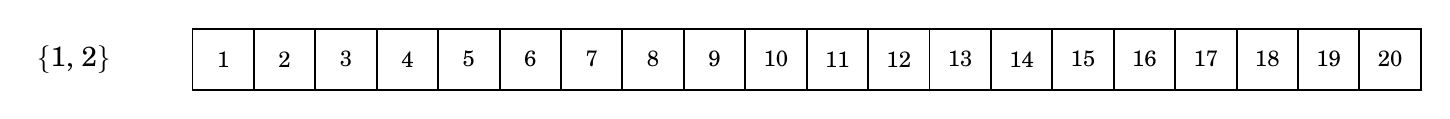
\begin{tikzpicture}
\node[anchor=west] at (0,-0.390) {\{1, 2\}};
\draw[line width=0.7pt] (2.100,0) rectangle (2.880,-0.780);
\node[font=\footnotesize] at (2.490,-0.390) {1};
\draw[line width=0.7pt] (2.880,0) rectangle (3.660,-0.780);
\node[font=\footnotesize] at (3.270,-0.390) {2};
\draw[line width=0.7pt] (3.660,0) rectangle (4.440,-0.780);
\node[font=\footnotesize] at (4.050,-0.390) {3};
\draw[line width=0.7pt] (4.440,0) rectangle (5.220,-0.780);
\node[font=\footnotesize] at (4.830,-0.390) {4};
\draw[line width=0.7pt] (5.220,0) rectangle (6.000,-0.780);
\node[font=\footnotesize] at (5.610,-0.390) {5};
\draw[line width=0.7pt] (6.000,0) rectangle (6.780,-0.780);
\node[font=\footnotesize] at (6.390,-0.390) {6};
\draw[line width=0.7pt] (6.780,0) rectangle (7.560,-0.780);
\node[font=\footnotesize] at (7.170,-0.390) {7};
\draw[line width=0.7pt] (7.560,0) rectangle (8.340,-0.780);
\node[font=\footnotesize] at (7.950,-0.390) {8};
\draw[line width=0.7pt] (8.340,0) rectangle (9.120,-0.780);
\node[font=\footnotesize] at (8.730,-0.390) {9};
\draw[line width=0.7pt] (9.120,0) rectangle (9.900,-0.780);
\node[font=\footnotesize] at (9.510,-0.390) {10};
\draw[line width=0.7pt] (9.900,0) rectangle (10.680,-0.780);
\node[font=\footnotesize] at (10.290,-0.390) {11};
\draw[line width=0.7pt] (10.680,0) rectangle (11.460,-0.780);
\node[font=\footnotesize] at (11.070,-0.390) {12};
\draw[line width=0.7pt] (11.460,0) rectangle (12.240,-0.780);
\node[font=\footnotesize] at (11.850,-0.390) {13};
\draw[line width=0.7pt] (12.240,0) rectangle (13.020,-0.780);
\node[font=\footnotesize] at (12.630,-0.390) {14};
\draw[line width=0.7pt] (13.020,0) rectangle (13.800,-0.780);
\node[font=\footnotesize] at (13.410,-0.390) {15};
\draw[line width=0.7pt] (13.800,0) rectangle (14.580,-0.780);
\node[font=\footnotesize] at (14.190,-0.390) {16};
\draw[line width=0.7pt] (14.580,0) rectangle (15.360,-0.780);
\node[font=\footnotesize] at (14.970,-0.390) {17};
\draw[line width=0.7pt] (15.360,0) rectangle (16.140,-0.780);
\node[font=\footnotesize] at (15.750,-0.390) {18};
\draw[line width=0.7pt] (16.140,0) rectangle (16.920,-0.780);
\node[font=\footnotesize] at (16.530,-0.390) {19};
\draw[line width=0.7pt] (16.920,0) rectangle (17.700,-0.780);
\node[font=\footnotesize] at (17.310,-0.390) {20};
\end{tikzpicture}

\vspace{2.4cm}
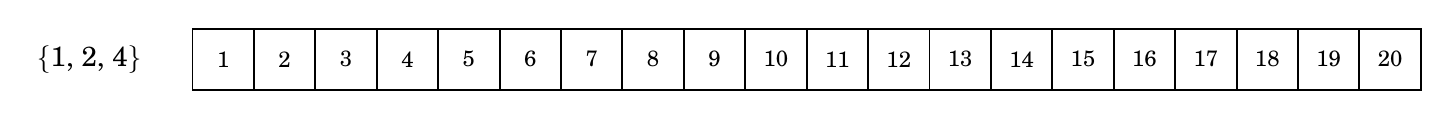
\begin{tikzpicture}
\node[anchor=west] at (0,-0.390) {\{1, 2, 4\}};
\draw[line width=0.7pt] (2.100,0) rectangle (2.880,-0.780);
\node[font=\footnotesize] at (2.490,-0.390) {1};
\draw[line width=0.7pt] (2.880,0) rectangle (3.660,-0.780);
\node[font=\footnotesize] at (3.270,-0.390) {2};
\draw[line width=0.7pt] (3.660,0) rectangle (4.440,-0.780);
\node[font=\footnotesize] at (4.050,-0.390) {3};
\draw[line width=0.7pt] (4.440,0) rectangle (5.220,-0.780);
\node[font=\footnotesize] at (4.830,-0.390) {4};
\draw[line width=0.7pt] (5.220,0) rectangle (6.000,-0.780);
\node[font=\footnotesize] at (5.610,-0.390) {5};
\draw[line width=0.7pt] (6.000,0) rectangle (6.780,-0.780);
\node[font=\footnotesize] at (6.390,-0.390) {6};
\draw[line width=0.7pt] (6.780,0) rectangle (7.560,-0.780);
\node[font=\footnotesize] at (7.170,-0.390) {7};
\draw[line width=0.7pt] (7.560,0) rectangle (8.340,-0.780);
\node[font=\footnotesize] at (7.950,-0.390) {8};
\draw[line width=0.7pt] (8.340,0) rectangle (9.120,-0.780);
\node[font=\footnotesize] at (8.730,-0.390) {9};
\draw[line width=0.7pt] (9.120,0) rectangle (9.900,-0.780);
\node[font=\footnotesize] at (9.510,-0.390) {10};
\draw[line width=0.7pt] (9.900,0) rectangle (10.680,-0.780);
\node[font=\footnotesize] at (10.290,-0.390) {11};
\draw[line width=0.7pt] (10.680,0) rectangle (11.460,-0.780);
\node[font=\footnotesize] at (11.070,-0.390) {12};
\draw[line width=0.7pt] (11.460,0) rectangle (12.240,-0.780);
\node[font=\footnotesize] at (11.850,-0.390) {13};
\draw[line width=0.7pt] (12.240,0) rectangle (13.020,-0.780);
\node[font=\footnotesize] at (12.630,-0.390) {14};
\draw[line width=0.7pt] (13.020,0) rectangle (13.800,-0.780);
\node[font=\footnotesize] at (13.410,-0.390) {15};
\draw[line width=0.7pt] (13.800,0) rectangle (14.580,-0.780);
\node[font=\footnotesize] at (14.190,-0.390) {16};
\draw[line width=0.7pt] (14.580,0) rectangle (15.360,-0.780);
\node[font=\footnotesize] at (14.970,-0.390) {17};
\draw[line width=0.7pt] (15.360,0) rectangle (16.140,-0.780);
\node[font=\footnotesize] at (15.750,-0.390) {18};
\draw[line width=0.7pt] (16.140,0) rectangle (16.920,-0.780);
\node[font=\footnotesize] at (16.530,-0.390) {19};
\draw[line width=0.7pt] (16.920,0) rectangle (17.700,-0.780);
\node[font=\footnotesize] at (17.310,-0.390) {20};
\end{tikzpicture}

\vspace{2.4cm}
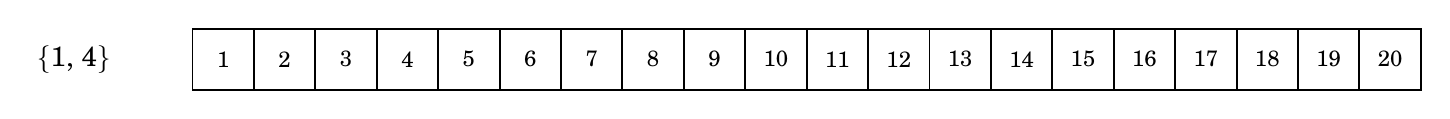
\begin{tikzpicture}
\node[anchor=west] at (0,-0.390) {\{1, 4\}};
\draw[line width=0.7pt] (2.100,0) rectangle (2.880,-0.780);
\node[font=\footnotesize] at (2.490,-0.390) {1};
\draw[line width=0.7pt] (2.880,0) rectangle (3.660,-0.780);
\node[font=\footnotesize] at (3.270,-0.390) {2};
\draw[line width=0.7pt] (3.660,0) rectangle (4.440,-0.780);
\node[font=\footnotesize] at (4.050,-0.390) {3};
\draw[line width=0.7pt] (4.440,0) rectangle (5.220,-0.780);
\node[font=\footnotesize] at (4.830,-0.390) {4};
\draw[line width=0.7pt] (5.220,0) rectangle (6.000,-0.780);
\node[font=\footnotesize] at (5.610,-0.390) {5};
\draw[line width=0.7pt] (6.000,0) rectangle (6.780,-0.780);
\node[font=\footnotesize] at (6.390,-0.390) {6};
\draw[line width=0.7pt] (6.780,0) rectangle (7.560,-0.780);
\node[font=\footnotesize] at (7.170,-0.390) {7};
\draw[line width=0.7pt] (7.560,0) rectangle (8.340,-0.780);
\node[font=\footnotesize] at (7.950,-0.390) {8};
\draw[line width=0.7pt] (8.340,0) rectangle (9.120,-0.780);
\node[font=\footnotesize] at (8.730,-0.390) {9};
\draw[line width=0.7pt] (9.120,0) rectangle (9.900,-0.780);
\node[font=\footnotesize] at (9.510,-0.390) {10};
\draw[line width=0.7pt] (9.900,0) rectangle (10.680,-0.780);
\node[font=\footnotesize] at (10.290,-0.390) {11};
\draw[line width=0.7pt] (10.680,0) rectangle (11.460,-0.780);
\node[font=\footnotesize] at (11.070,-0.390) {12};
\draw[line width=0.7pt] (11.460,0) rectangle (12.240,-0.780);
\node[font=\footnotesize] at (11.850,-0.390) {13};
\draw[line width=0.7pt] (12.240,0) rectangle (13.020,-0.780);
\node[font=\footnotesize] at (12.630,-0.390) {14};
\draw[line width=0.7pt] (13.020,0) rectangle (13.800,-0.780);
\node[font=\footnotesize] at (13.410,-0.390) {15};
\draw[line width=0.7pt] (13.800,0) rectangle (14.580,-0.780);
\node[font=\footnotesize] at (14.190,-0.390) {16};
\draw[line width=0.7pt] (14.580,0) rectangle (15.360,-0.780);
\node[font=\footnotesize] at (14.970,-0.390) {17};
\draw[line width=0.7pt] (15.360,0) rectangle (16.140,-0.780);
\node[font=\footnotesize] at (15.750,-0.390) {18};
\draw[line width=0.7pt] (16.140,0) rectangle (16.920,-0.780);
\node[font=\footnotesize] at (16.530,-0.390) {19};
\draw[line width=0.7pt] (16.920,0) rectangle (17.700,-0.780);
\node[font=\footnotesize] at (17.310,-0.390) {20};
\end{tikzpicture}

\vspace{2.4cm}
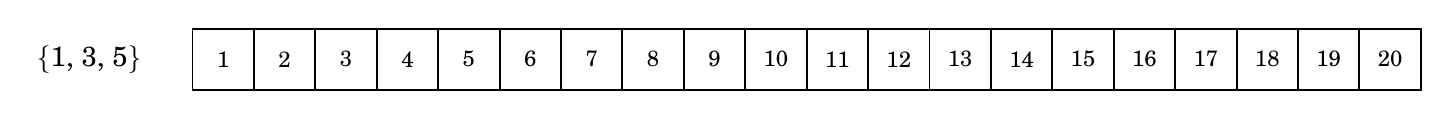
\begin{tikzpicture}
\node[anchor=west] at (0,-0.390) {\{1, 3, 5\}};
\draw[line width=0.7pt] (2.100,0) rectangle (2.880,-0.780);
\node[font=\footnotesize] at (2.490,-0.390) {1};
\draw[line width=0.7pt] (2.880,0) rectangle (3.660,-0.780);
\node[font=\footnotesize] at (3.270,-0.390) {2};
\draw[line width=0.7pt] (3.660,0) rectangle (4.440,-0.780);
\node[font=\footnotesize] at (4.050,-0.390) {3};
\draw[line width=0.7pt] (4.440,0) rectangle (5.220,-0.780);
\node[font=\footnotesize] at (4.830,-0.390) {4};
\draw[line width=0.7pt] (5.220,0) rectangle (6.000,-0.780);
\node[font=\footnotesize] at (5.610,-0.390) {5};
\draw[line width=0.7pt] (6.000,0) rectangle (6.780,-0.780);
\node[font=\footnotesize] at (6.390,-0.390) {6};
\draw[line width=0.7pt] (6.780,0) rectangle (7.560,-0.780);
\node[font=\footnotesize] at (7.170,-0.390) {7};
\draw[line width=0.7pt] (7.560,0) rectangle (8.340,-0.780);
\node[font=\footnotesize] at (7.950,-0.390) {8};
\draw[line width=0.7pt] (8.340,0) rectangle (9.120,-0.780);
\node[font=\footnotesize] at (8.730,-0.390) {9};
\draw[line width=0.7pt] (9.120,0) rectangle (9.900,-0.780);
\node[font=\footnotesize] at (9.510,-0.390) {10};
\draw[line width=0.7pt] (9.900,0) rectangle (10.680,-0.780);
\node[font=\footnotesize] at (10.290,-0.390) {11};
\draw[line width=0.7pt] (10.680,0) rectangle (11.460,-0.780);
\node[font=\footnotesize] at (11.070,-0.390) {12};
\draw[line width=0.7pt] (11.460,0) rectangle (12.240,-0.780);
\node[font=\footnotesize] at (11.850,-0.390) {13};
\draw[line width=0.7pt] (12.240,0) rectangle (13.020,-0.780);
\node[font=\footnotesize] at (12.630,-0.390) {14};
\draw[line width=0.7pt] (13.020,0) rectangle (13.800,-0.780);
\node[font=\footnotesize] at (13.410,-0.390) {15};
\draw[line width=0.7pt] (13.800,0) rectangle (14.580,-0.780);
\node[font=\footnotesize] at (14.190,-0.390) {16};
\draw[line width=0.7pt] (14.580,0) rectangle (15.360,-0.780);
\node[font=\footnotesize] at (14.970,-0.390) {17};
\draw[line width=0.7pt] (15.360,0) rectangle (16.140,-0.780);
\node[font=\footnotesize] at (15.750,-0.390) {18};
\draw[line width=0.7pt] (16.140,0) rectangle (16.920,-0.780);
\node[font=\footnotesize] at (16.530,-0.390) {19};
\draw[line width=0.7pt] (16.920,0) rectangle (17.700,-0.780);
\node[font=\footnotesize] at (17.310,-0.390) {20};
\end{tikzpicture}
\vspace{2.4cm}
\end{problem}
\begin{problem}
\prob{4} Dana's plan is to always take as many counters as the rule allows. In which of the games \game{1, 2}, \game{1, 3, 4}, \game{1, 4}, and \game{1, 3, 5} does Dana's plan always win when she starts at a winning pile? For each game where it does not, find a winning pile where the plan loses against good play. For each game where it does, explain why it always wins.
\begin{center}
\renewcommand{\arraystretch}{1.25}
\begin{tabular}{|>{\centering\arraybackslash}m{3.2cm}|>{\centering\arraybackslash}m{5.0cm}|>{\centering\arraybackslash}m{5.6cm}|}
\hline
Game & Does the plan always win? & A winning pile where it loses \\ \hline
\{1, 2\}\rule[-0.42cm]{0pt}{1.15cm} &  &  \\ \hline
\{1, 3, 4\}\rule[-0.42cm]{0pt}{1.15cm} &  &  \\ \hline
\{1, 4\}\rule[-0.42cm]{0pt}{1.15cm} &  &  \\ \hline
\{1, 3, 5\}\rule[-0.42cm]{0pt}{1.15cm} &  &  \\ \hline
\end{tabular}
\end{center}
\vspace{5.0cm}
\end{problem}
\begin{problem}
\prob{5} Explain why the pattern of losing piles you found in Problem 1 must keep going forever, for piles of every size.
\vspace{8.0cm}
\end{problem}
\begin{problem}
\prob{6} Find every game whose allowed moves come from the numbers 1, 2, 3, 4, 5, and 6 and whose losing piles are exactly the multiples of 4. Explain why your list is complete.
\vspace{9.0cm}
\end{problem}
\begin{problem}
\prob{7} Change the rule so that whoever takes the last counter loses. Shade the losing piles from 1 to 20 in the \game{1, 2} game and in the \game{1, 3, 4} game with this new rule. Compare them with the losing piles you found when taking the last counter wins, and explain the difference.
\vspace{0.4cm}

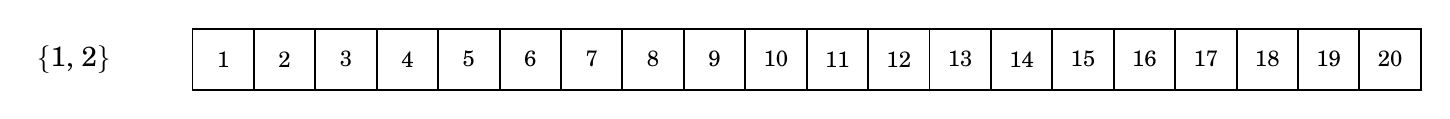
\begin{tikzpicture}
\node[anchor=west] at (0,-0.390) {\{1, 2\}};
\draw[line width=0.7pt] (2.100,0) rectangle (2.880,-0.780);
\node[font=\footnotesize] at (2.490,-0.390) {1};
\draw[line width=0.7pt] (2.880,0) rectangle (3.660,-0.780);
\node[font=\footnotesize] at (3.270,-0.390) {2};
\draw[line width=0.7pt] (3.660,0) rectangle (4.440,-0.780);
\node[font=\footnotesize] at (4.050,-0.390) {3};
\draw[line width=0.7pt] (4.440,0) rectangle (5.220,-0.780);
\node[font=\footnotesize] at (4.830,-0.390) {4};
\draw[line width=0.7pt] (5.220,0) rectangle (6.000,-0.780);
\node[font=\footnotesize] at (5.610,-0.390) {5};
\draw[line width=0.7pt] (6.000,0) rectangle (6.780,-0.780);
\node[font=\footnotesize] at (6.390,-0.390) {6};
\draw[line width=0.7pt] (6.780,0) rectangle (7.560,-0.780);
\node[font=\footnotesize] at (7.170,-0.390) {7};
\draw[line width=0.7pt] (7.560,0) rectangle (8.340,-0.780);
\node[font=\footnotesize] at (7.950,-0.390) {8};
\draw[line width=0.7pt] (8.340,0) rectangle (9.120,-0.780);
\node[font=\footnotesize] at (8.730,-0.390) {9};
\draw[line width=0.7pt] (9.120,0) rectangle (9.900,-0.780);
\node[font=\footnotesize] at (9.510,-0.390) {10};
\draw[line width=0.7pt] (9.900,0) rectangle (10.680,-0.780);
\node[font=\footnotesize] at (10.290,-0.390) {11};
\draw[line width=0.7pt] (10.680,0) rectangle (11.460,-0.780);
\node[font=\footnotesize] at (11.070,-0.390) {12};
\draw[line width=0.7pt] (11.460,0) rectangle (12.240,-0.780);
\node[font=\footnotesize] at (11.850,-0.390) {13};
\draw[line width=0.7pt] (12.240,0) rectangle (13.020,-0.780);
\node[font=\footnotesize] at (12.630,-0.390) {14};
\draw[line width=0.7pt] (13.020,0) rectangle (13.800,-0.780);
\node[font=\footnotesize] at (13.410,-0.390) {15};
\draw[line width=0.7pt] (13.800,0) rectangle (14.580,-0.780);
\node[font=\footnotesize] at (14.190,-0.390) {16};
\draw[line width=0.7pt] (14.580,0) rectangle (15.360,-0.780);
\node[font=\footnotesize] at (14.970,-0.390) {17};
\draw[line width=0.7pt] (15.360,0) rectangle (16.140,-0.780);
\node[font=\footnotesize] at (15.750,-0.390) {18};
\draw[line width=0.7pt] (16.140,0) rectangle (16.920,-0.780);
\node[font=\footnotesize] at (16.530,-0.390) {19};
\draw[line width=0.7pt] (16.920,0) rectangle (17.700,-0.780);
\node[font=\footnotesize] at (17.310,-0.390) {20};
\end{tikzpicture}

\vspace{0.6cm}
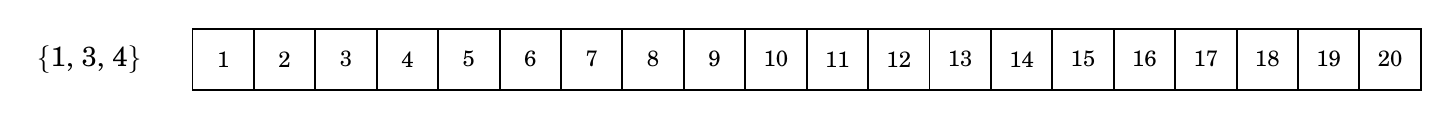
\begin{tikzpicture}
\node[anchor=west] at (0,-0.390) {\{1, 3, 4\}};
\draw[line width=0.7pt] (2.100,0) rectangle (2.880,-0.780);
\node[font=\footnotesize] at (2.490,-0.390) {1};
\draw[line width=0.7pt] (2.880,0) rectangle (3.660,-0.780);
\node[font=\footnotesize] at (3.270,-0.390) {2};
\draw[line width=0.7pt] (3.660,0) rectangle (4.440,-0.780);
\node[font=\footnotesize] at (4.050,-0.390) {3};
\draw[line width=0.7pt] (4.440,0) rectangle (5.220,-0.780);
\node[font=\footnotesize] at (4.830,-0.390) {4};
\draw[line width=0.7pt] (5.220,0) rectangle (6.000,-0.780);
\node[font=\footnotesize] at (5.610,-0.390) {5};
\draw[line width=0.7pt] (6.000,0) rectangle (6.780,-0.780);
\node[font=\footnotesize] at (6.390,-0.390) {6};
\draw[line width=0.7pt] (6.780,0) rectangle (7.560,-0.780);
\node[font=\footnotesize] at (7.170,-0.390) {7};
\draw[line width=0.7pt] (7.560,0) rectangle (8.340,-0.780);
\node[font=\footnotesize] at (7.950,-0.390) {8};
\draw[line width=0.7pt] (8.340,0) rectangle (9.120,-0.780);
\node[font=\footnotesize] at (8.730,-0.390) {9};
\draw[line width=0.7pt] (9.120,0) rectangle (9.900,-0.780);
\node[font=\footnotesize] at (9.510,-0.390) {10};
\draw[line width=0.7pt] (9.900,0) rectangle (10.680,-0.780);
\node[font=\footnotesize] at (10.290,-0.390) {11};
\draw[line width=0.7pt] (10.680,0) rectangle (11.460,-0.780);
\node[font=\footnotesize] at (11.070,-0.390) {12};
\draw[line width=0.7pt] (11.460,0) rectangle (12.240,-0.780);
\node[font=\footnotesize] at (11.850,-0.390) {13};
\draw[line width=0.7pt] (12.240,0) rectangle (13.020,-0.780);
\node[font=\footnotesize] at (12.630,-0.390) {14};
\draw[line width=0.7pt] (13.020,0) rectangle (13.800,-0.780);
\node[font=\footnotesize] at (13.410,-0.390) {15};
\draw[line width=0.7pt] (13.800,0) rectangle (14.580,-0.780);
\node[font=\footnotesize] at (14.190,-0.390) {16};
\draw[line width=0.7pt] (14.580,0) rectangle (15.360,-0.780);
\node[font=\footnotesize] at (14.970,-0.390) {17};
\draw[line width=0.7pt] (15.360,0) rectangle (16.140,-0.780);
\node[font=\footnotesize] at (15.750,-0.390) {18};
\draw[line width=0.7pt] (16.140,0) rectangle (16.920,-0.780);
\node[font=\footnotesize] at (16.530,-0.390) {19};
\draw[line width=0.7pt] (16.920,0) rectangle (17.700,-0.780);
\node[font=\footnotesize] at (17.310,-0.390) {20};
\end{tikzpicture}
\vspace{6.0cm}
\end{problem}
\begin{problem}
\prob{8} Now there are two piles. On each turn, a player takes 1 or 2 counters from one of the piles, and whoever takes the last counter on the table wins. In the grid, the square in row 3 and column 1 stands for a pile of 3 counters and a pile of 1 counter, and row 0 or column 0 stands for an empty pile. Shade every square where you would rather go second. When the two piles are the same size, which player can always win? Explain why.
\vspace{0.3cm}
\begin{center}
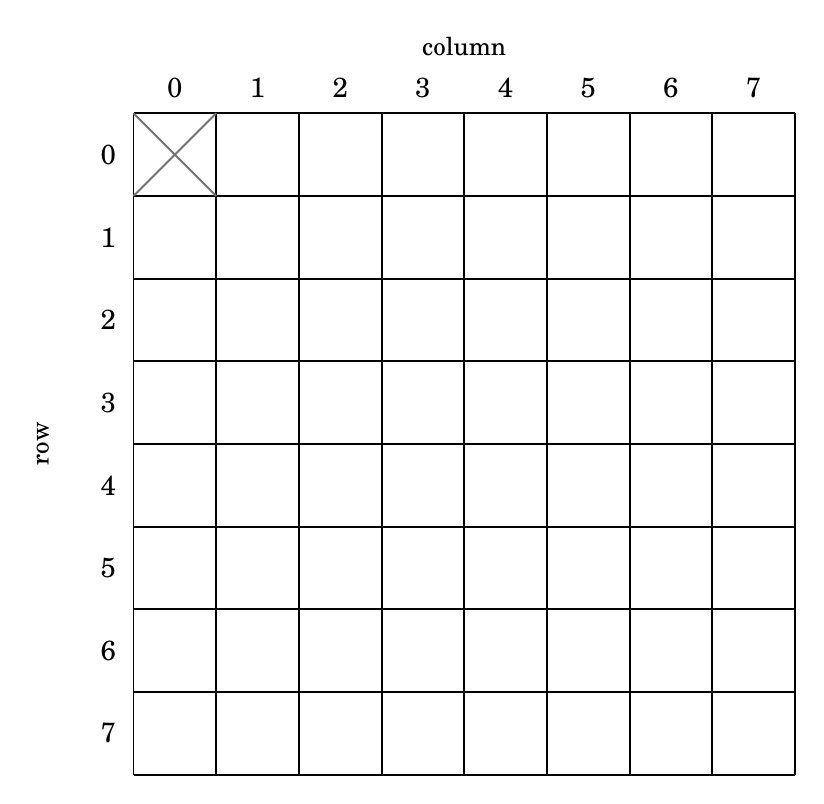
\begin{tikzpicture}
\draw[line width=0.7pt] (0,0.000) -- (8.400,0.000);
\draw[line width=0.7pt] (0.000,0) -- (0.000,-8.400);
\draw[line width=0.7pt] (0,-1.050) -- (8.400,-1.050);
\draw[line width=0.7pt] (1.050,0) -- (1.050,-8.400);
\draw[line width=0.7pt] (0,-2.100) -- (8.400,-2.100);
\draw[line width=0.7pt] (2.100,0) -- (2.100,-8.400);
\draw[line width=0.7pt] (0,-3.150) -- (8.400,-3.150);
\draw[line width=0.7pt] (3.150,0) -- (3.150,-8.400);
\draw[line width=0.7pt] (0,-4.200) -- (8.400,-4.200);
\draw[line width=0.7pt] (4.200,0) -- (4.200,-8.400);
\draw[line width=0.7pt] (0,-5.250) -- (8.400,-5.250);
\draw[line width=0.7pt] (5.250,0) -- (5.250,-8.400);
\draw[line width=0.7pt] (0,-6.300) -- (8.400,-6.300);
\draw[line width=0.7pt] (6.300,0) -- (6.300,-8.400);
\draw[line width=0.7pt] (0,-7.350) -- (8.400,-7.350);
\draw[line width=0.7pt] (7.350,0) -- (7.350,-8.400);
\draw[line width=0.7pt] (0,-8.400) -- (8.400,-8.400);
\draw[line width=0.7pt] (8.400,0) -- (8.400,-8.400);
\draw[black!55,line width=0.7pt] (0,0) -- (1.050,-1.050) (0,-1.050) -- (1.050,0);
\node at (0.525,0.32) {0};
\node at (-0.32,-0.525) {0};
\node at (1.575,0.32) {1};
\node at (-0.32,-1.575) {1};
\node at (2.625,0.32) {2};
\node at (-0.32,-2.625) {2};
\node at (3.675,0.32) {3};
\node at (-0.32,-3.675) {3};
\node at (4.725,0.32) {4};
\node at (-0.32,-4.725) {4};
\node at (5.775,0.32) {5};
\node at (-0.32,-5.775) {5};
\node at (6.825,0.32) {6};
\node at (-0.32,-6.825) {6};
\node at (7.875,0.32) {7};
\node at (-0.32,-7.875) {7};
\node[font=\small] at (4.200,0.85) {column};
\node[font=\small,rotate=90] at (-1.15,-4.200) {row};
\end{tikzpicture}
\end{center}

\vspace{4.0cm}
\end{problem}
\begin{problem}
\prob{9} Play the two-pile game again, but now each move takes 1, 3, or 4 counters from one of the piles. Find every pair of piles of different sizes, each with 1 to 8 counters, where you would rather go second. The grid works the same way as in Problem 8.
\vspace{0.3cm}
\begin{center}
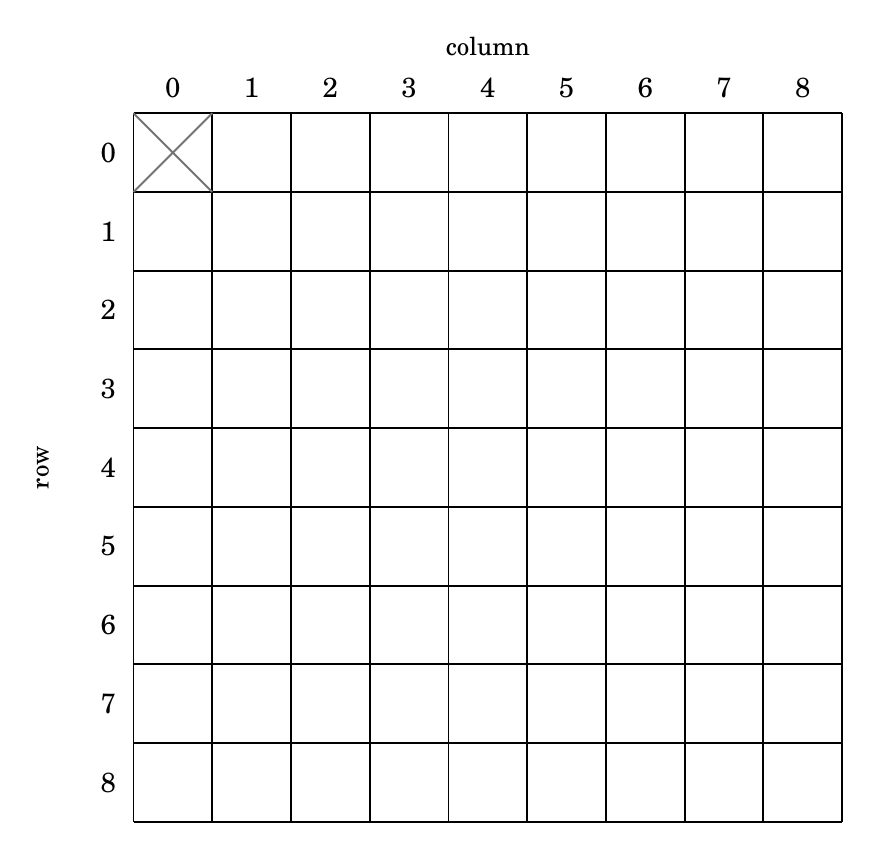
\begin{tikzpicture}
\draw[line width=0.7pt] (0,0.000) -- (9.000,0.000);
\draw[line width=0.7pt] (0.000,0) -- (0.000,-9.000);
\draw[line width=0.7pt] (0,-1.000) -- (9.000,-1.000);
\draw[line width=0.7pt] (1.000,0) -- (1.000,-9.000);
\draw[line width=0.7pt] (0,-2.000) -- (9.000,-2.000);
\draw[line width=0.7pt] (2.000,0) -- (2.000,-9.000);
\draw[line width=0.7pt] (0,-3.000) -- (9.000,-3.000);
\draw[line width=0.7pt] (3.000,0) -- (3.000,-9.000);
\draw[line width=0.7pt] (0,-4.000) -- (9.000,-4.000);
\draw[line width=0.7pt] (4.000,0) -- (4.000,-9.000);
\draw[line width=0.7pt] (0,-5.000) -- (9.000,-5.000);
\draw[line width=0.7pt] (5.000,0) -- (5.000,-9.000);
\draw[line width=0.7pt] (0,-6.000) -- (9.000,-6.000);
\draw[line width=0.7pt] (6.000,0) -- (6.000,-9.000);
\draw[line width=0.7pt] (0,-7.000) -- (9.000,-7.000);
\draw[line width=0.7pt] (7.000,0) -- (7.000,-9.000);
\draw[line width=0.7pt] (0,-8.000) -- (9.000,-8.000);
\draw[line width=0.7pt] (8.000,0) -- (8.000,-9.000);
\draw[line width=0.7pt] (0,-9.000) -- (9.000,-9.000);
\draw[line width=0.7pt] (9.000,0) -- (9.000,-9.000);
\draw[black!55,line width=0.7pt] (0,0) -- (1.000,-1.000) (0,-1.000) -- (1.000,0);
\node at (0.500,0.32) {0};
\node at (-0.32,-0.500) {0};
\node at (1.500,0.32) {1};
\node at (-0.32,-1.500) {1};
\node at (2.500,0.32) {2};
\node at (-0.32,-2.500) {2};
\node at (3.500,0.32) {3};
\node at (-0.32,-3.500) {3};
\node at (4.500,0.32) {4};
\node at (-0.32,-4.500) {4};
\node at (5.500,0.32) {5};
\node at (-0.32,-5.500) {5};
\node at (6.500,0.32) {6};
\node at (-0.32,-6.500) {6};
\node at (7.500,0.32) {7};
\node at (-0.32,-7.500) {7};
\node at (8.500,0.32) {8};
\node at (-0.32,-8.500) {8};
\node[font=\small] at (4.500,0.85) {column};
\node[font=\small,rotate=90] at (-1.15,-4.500) {row};
\end{tikzpicture}
\end{center}

\vspace{2.0cm}
\end{problem}
\end{document}
